\documentclass[12pt]{article}

\usepackage{sbc-template}
\usepackage{graphicx,url}
\usepackage[utf8]{inputenc}
\usepackage[brazil]{babel}
\title{Algoritmos de Busca no Pac-Man \\
Introdução à Inteligência Artificial}

\author{Vinicius Julião Ramos - 2018054630}


\address{Departamento de Ciência da Computação \\Universidade Federal de Minas Gerais
(UFMG)
\email{viniciusjuliao@dcc.ufmg.br}
}

\begin{document} 
\maketitle


\section{Introdução}

O presente trabalho constituído pelo desenvolvimento e análise da aplicação
de algoritmos de busca sobre o jogo Pac-Man.
Essa atividade tem como fim a introdução de algoritmos utilizados por
inteligências artificiais em problemas reais, como um \textit{video game}.
Além disso, tal aplicação só é possível graças à modelagem do problema, em que
o estado do jogo se dá pelas posições disponíveis no tabuleiro (mapa),
sendo que os estados considerados como estados objetivos, são aqueles que
contêm a "comida" do personagem.

No jogo, o personagem pode mudar de posição apenas para aquelas posições
ajacentes à posição atual.
Tal adjacência se dá pelas posições acima, abaixo, à esquerda e à direita.
Logo, cada estado tem no máximo quatro outros estados descendentes.
É importante destacar que o mapa não é infinito, ou seja, há barreiras que
impedem o personagem de realizar um movimento, logo é possível que
determinados estados tenham menos de quatro estados descendentes.
Dessa forma, é possível caminhar de forma sistêmica em todo este grafo a fim
de alcançar os estados objetivos, e vencer o jogo.

Apesar da simplicidade do solucionador de um jogo 2D, a busca em grafos é
utilizada em diversas aplicações muito complexas, mas, em linhas gerais, tem
implementação relativamente simples.
Outro fator de importância dos algoritmos de busca, é à adaptabilidade para
diferentes tipos de problemas, enquanto há aqueles que são aplicáveis a
qualquer problema, há outros que demandam maior conversão de especificidade.
Um bom exemplo são os algoritmos \textbf{BFS} e \textbf{A*}, no qual o primeiro
pode ser aplicado de maneira genérica em muitos tipos de busca em grafos.
Já o segundo algoritmo, demanda a criação de uma função heurística, o que
desperta a necessidade de entender do comportamento das instancias
que o algoritmo resolve, a fim de que essa função heurística seja capaz
de optimizar a busca.

\section{Soluções}
De maneira geral, como trata-se de buscas em grafos, este tralho desenvolveu
três estruturas diferentes de solucionadores que serão apresentadas em
ordem a seguir.
As duas primeiras, são buscas que não desconsideram custos na troca de estados,
entretanto, cada uma delas tem a própria maneira de expansão de nós.
Já a ultima estrutura, que fora utilizada para três algoritmos diferentes,
atribui pesos às mudanças de estado de maneira a optimizar -- minimizar --
a quantidade de nós expandidos.

\subsection{Busca em Profundidade}
Este é um algoritmo recursivo, que não considera custos de transições de
estado, assim como mostram \cite{stuart:00} e \cite{cormen:01}.
A composição algorítmica desta solução, faz com que a partir de um determinado
nó, de maneira recursiva, visite-se imediatamente os nós vizinhos (que ainda
não foram visitados).
Ao imaginar uma árvore de decisão, em que os nós da árvore são os estados do
problema e as arestas são as decisões de transições tomadas pelo algoritmo,
a busca em profundidade parte da raiz (estado inicial) visitando primeiramente
todo um ramo da árvore, antes de visitar quaisquer outros nós.
Ao se deparar com um nó folha, atinge-se a condição de parada da recursão,
e então, parte-se para a visitação do \textit{sub-ramo} que descende do pai
daquele nó folha.
Contanto, a condição de parada que o algoritmo busca é o nó que identifica
o estado objetivo do problema.
Ao alcançar este ponto, o algoritmo é finalizado.

Apesar da característica recursiva do problema, o código desta solução não
foi desenvolvido com chamadas recursivas.
É possível utilizar uma estrutura de \textbf{pilha} para a visitação em
profundidade, então optou-se por esta solução, uma vez que o empilhamento
de chamadas recursivas adiciona uma sobrecarga muito grande na solução.
Em instancias muito grandes, a árvore de decisões pode conter diversos níveis
e para cada nível, adicionaria-se uma chamada de função, sobrecarregando
a solução com a criação de novas variáveis.
A solução chamada iterativa, necessita apenas de armazenar os dados de cada
nó (estado) que será visitado a posteriori.

Por fim, utilizou-se também uma segunda pilha para armazenar a sequencia de
tomadas de decisão realizadas pela busca em profundidade.
Cada vez que a solução se aprofunda um nível da árvore de decisões, armazena-ze
aquele aprofundamento.
Da mesma maneira, ao voltar um nível (emergir), a ultima decisão armazenada
na pilha é removida.
Enfim, ao encontrar o nó objetivo e parar a busca em profundidade, a pilha
de decisões armazenou o passo a passo de como sair do nó raiz e chegar até
o objetivo.

\subsection{Busca em Largura}
Em contraste com a busca em profundidade, nesta solução, a visitação
da árvore de decisão é realizada de maneira "ramo a ramo".
Na verdade, deseja-se visitar a árvore de decisões nível a nível.
Ou seja, para que um nível $i+1$ seja visitado, é necessário que todos
os nós do nível $i$ já tenham sido visitados anteriormente.
A implementação dessa característica de visitação, requer o uso de uma
estrutura de \textbf{fila}, em que, ao visitar um nó $n$, adiciona-se
ao final da fila todos os nós filhos de $n$.
Em questões práticas, ao expandir o estado $s$, todos os estados vizinhos
de $s$ são adicionados ao fim da fila.

Através dessa expansão em largura, pode-se chegar até o nó objetivo.
Contudo, é preciso lembrar de uma restrição que fora adicionada a todas
as soluções: Um estado não deve se expandido mais de uma vez, ou seja,
na árvore de decisões não visitamos o mesmo nó mais de uma vez.
Diferentemente da visitação em profundidade, a qual a própria pilha de
visitação armazena as transições que a solução deve apresentar,
na busca em largura é necessário utilizar uma estrutura mais complexa.
Optou-se pela implementação de um dicionário, no qual, após expandir
determinado nó, armazenamos aquele nó no dicionário, mapeando o
nó pai.
Dessa maneira, para obter a sequencia de decisões (a solução), desde que o
nó objetivo fosse encontrado, bastou caminhar no dicionário em
direção ao nó raiz da árvore de decisões.

\subsection{Busca em Transições Ponderadas}
As outras três soluções apresentadas por este trabalho consideram o peso
da transições ou pesos dos estados ao realizar a visitação dos nós da árvore
de decisão.
Estes algoritmos são \textbf{A*}, \textbf{Greedy}, e
\textbf{Uniform Cost Search}, os quais possuem a mesma estrutura básica, sendo
que a única mudança é a função que avalia a qualidade da transição, assim como
mostrado em \cite{stuart:00}.

Neste ponto, houve a necessidade de utilizar a estrutura
\textbf{fila de prioridades}, na qual a função \textit{custo de transição}
define a ordem de expansão dos estados.
Ou seja, cada vez que um estado é expandido, os estados vizinhos são
adicionados à fila de prioridades, sendo que o \textit{custo de transição}
é definido pelo respectivo algoritmo, dentre aqueles três que realizam
tal ponderação.
Exatamente como na busca em largura, a estrutura de dicionário também fora
utilizada para armazenar a sequência de visitação.
Assim que um nó é visitado, ele é adicionado ao dicionário mapeando o nó
predecessor.
Ao encontra o nó objetivo, basta caminhar no dicionário em direção
ao nó raiz (estado inicial).

\section{Metodologia e Análise Experimental}
Para a análise experimental, optou-se pela utilização das métrica retornadas
pelos códigos previamente escritos em que temos o tempo de execução, a
quantidade de nós expandidos e o custo da solução.
A obtenção dessa métricas se deu por meio do seguinte comando:

\begin{center}
  \textit{python3 pacman.py --layout \$scenario --pacman SearchAgent --agentArgs fn=\$alg,prob=FoodSearchProblem,heuristic=foodHeuristic}
\end{center}

Observe, que o comando utiliza a heurística desenvolvida por este trabalho.
Além disso, dadas as duas variáveis contidas no comando, executou-se todas as
combinações possíveis de \textit{\$scenaio, \$alg}.
As quais contiveram os seguintes valores:
\begin{itemize}
  \item \textbf{\textit{\$alg}}: \textit{dfs} $|$ \textit{bfs} $|$ \textit{ucs} $|$ \textit{gs}
  $|$ \textit{astar}
  \item \textbf{\textit{\$scenario}}: \textit{contoursMaze} $|$ \textit{greedySearch} $|$
  \textit{mediumCorners} $|$ \textit{mediumSafeSearch} $|$ \textit{openMaze} $|$
  \textit{smallMaze} $|$ \textit{smallSafeSearch} $|$ \textit{smallSearch} $|$
  \textit{tinyCorners} $|$ \textit{trickySearch}
\end{itemize}

\subsection{Desempenho de cada algoritmo}
Os resultados obtidos nesta fase da análise foram realizados de forma que
para cada \textit{\$alg} computou-se a média de execução das métricas em cada
\textit{\$scenario}.
Além disso, os dados foram normalizados e dessa forma, encontram-se numa escala
entre 0 e 1.

\begin{figure}[hbt!]
  \centering
  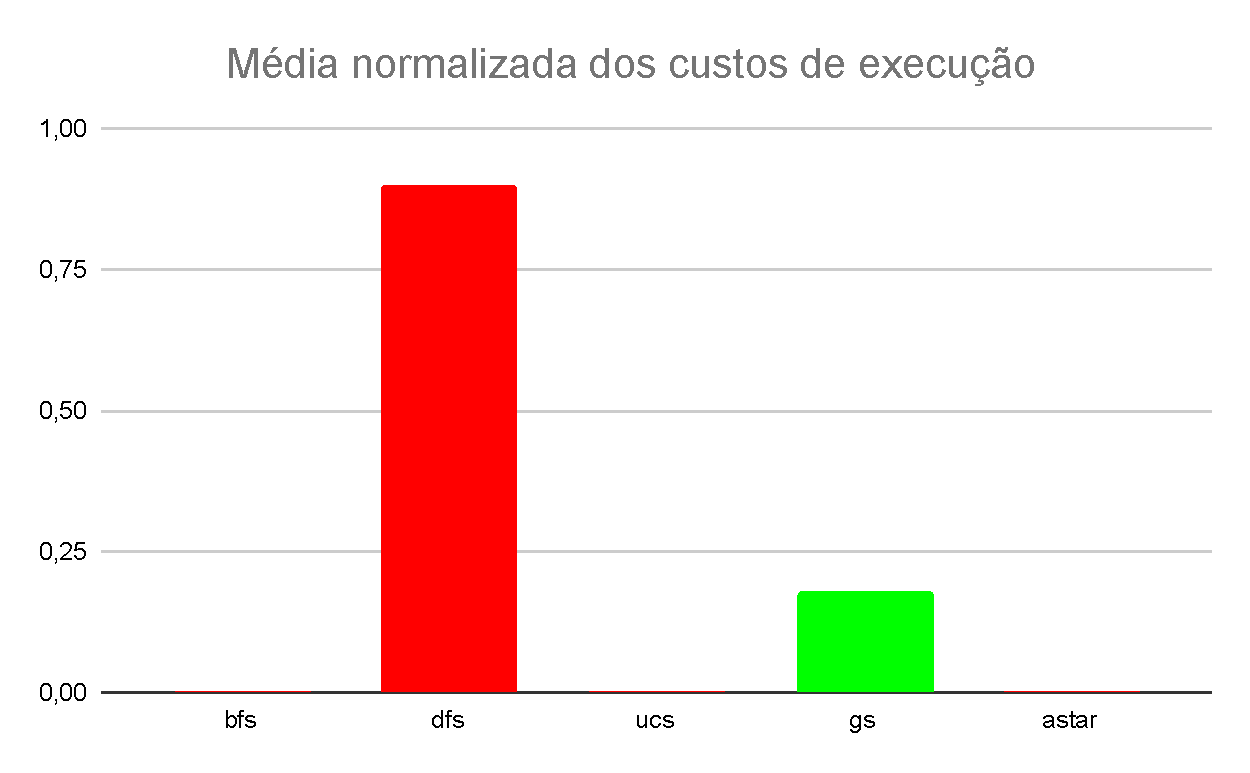
\includegraphics[width=.8\textwidth]{fig/custo.pdf}
  \caption{Média dos custos de execução de todos possíveis \textit{\$scenarios} para cada \textit{\$alg}.}
  \label{fig:custo}
\end{figure}

O alto custo do algoritmo \textit{dfs}, destacado na Figura~\ref{fig:custo} é
causado pela forma como a busca é realizada.
Nesta solução, o que ocorre é uma busca cega através do mapa do jogo, o que
pode levar a movimentos desnecessários, elevando o custo da solução.
Entretanto, este algoritmo possui uma grande vantagem observada nas Figuras
~\ref{fig:tempo} e ~\ref{fig:expansao}.
O tempo e a quantidade de nós expandidos estão entre os menores valores
dentre os cinco algoritmos analisados.
Sendo que há uma relação entre tais fatores, uma vez que pode-se atribuir ir o
baixo tempo à baixa quantidade de nós expandidos.
Tal relação também é rechaçada pelos algoritmos \textit{ucs} e \textit{astar}.

\begin{figure}[hbt!]
  \centering
  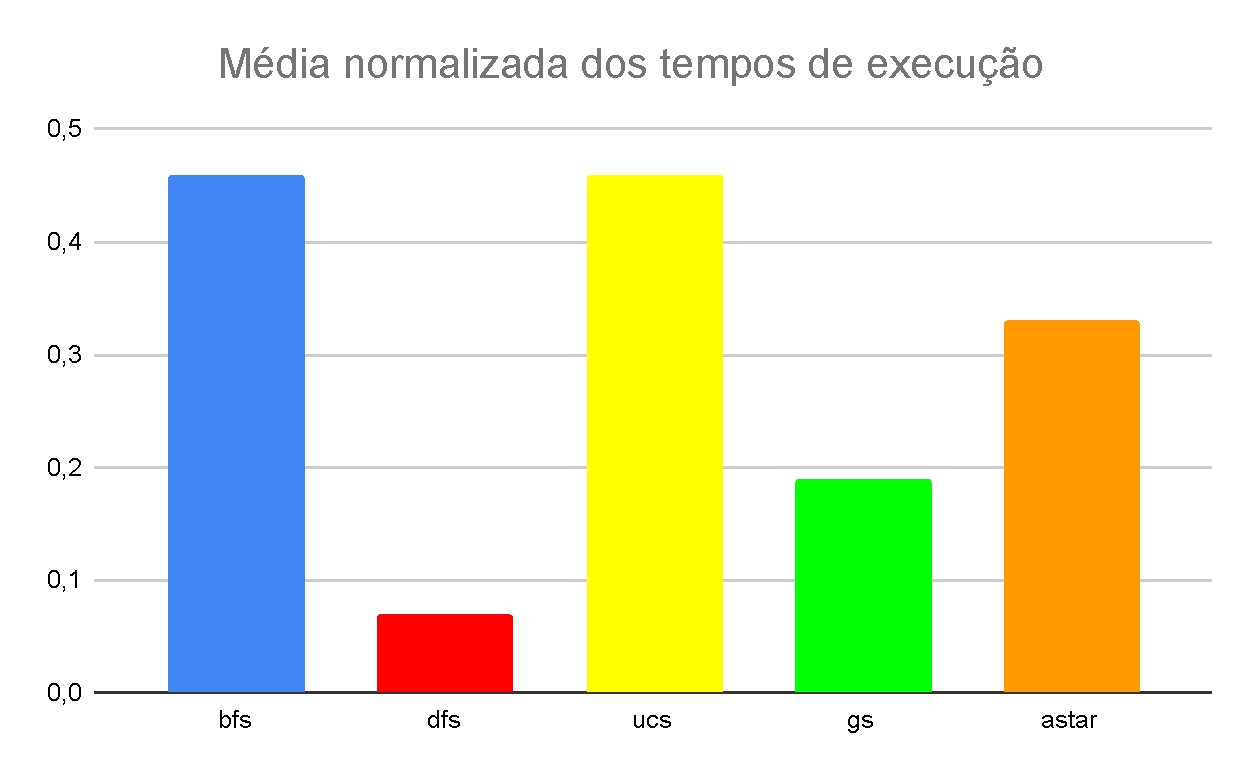
\includegraphics[width=.8\textwidth]{fig/tempo.pdf}
  \caption{Média dos tempos de execução de todos possíveis \textit{\$scenarios} para cada \textit{\$alg}.}
  \label{fig:tempo}
\end{figure}

Entretanto, ao analisar o desempenho de todos os algoritmos, é possível
confirmar o bom desempenho daqueles que utilizam heurísticas para
ponderar as transições.
Tanto \textit{gs} quanto \textit{astar} expandiram poucos nós e tiveram um baixo
tempo de execução.
Entretanto, enquanto \textit{astar} é melhor na custo médio das soluções, ele
também se saiu pior do que \textit{gs} nos fatores Tempo e Número de nós Expandidos.
Então, por vias práticas, é necessário realizar um \textit{trade-off} entre
melhor custo e melhor desempenho ao selecionar um destes dois algoritmos.
Isso comprova o que fora dito durante as aulas, que dentre os cinco
algoritmos, \textit{astar} é aquele que melhor se aproxima da optimalidade
com um bom desempenho.


\begin{figure}[hbt!]
  \centering
  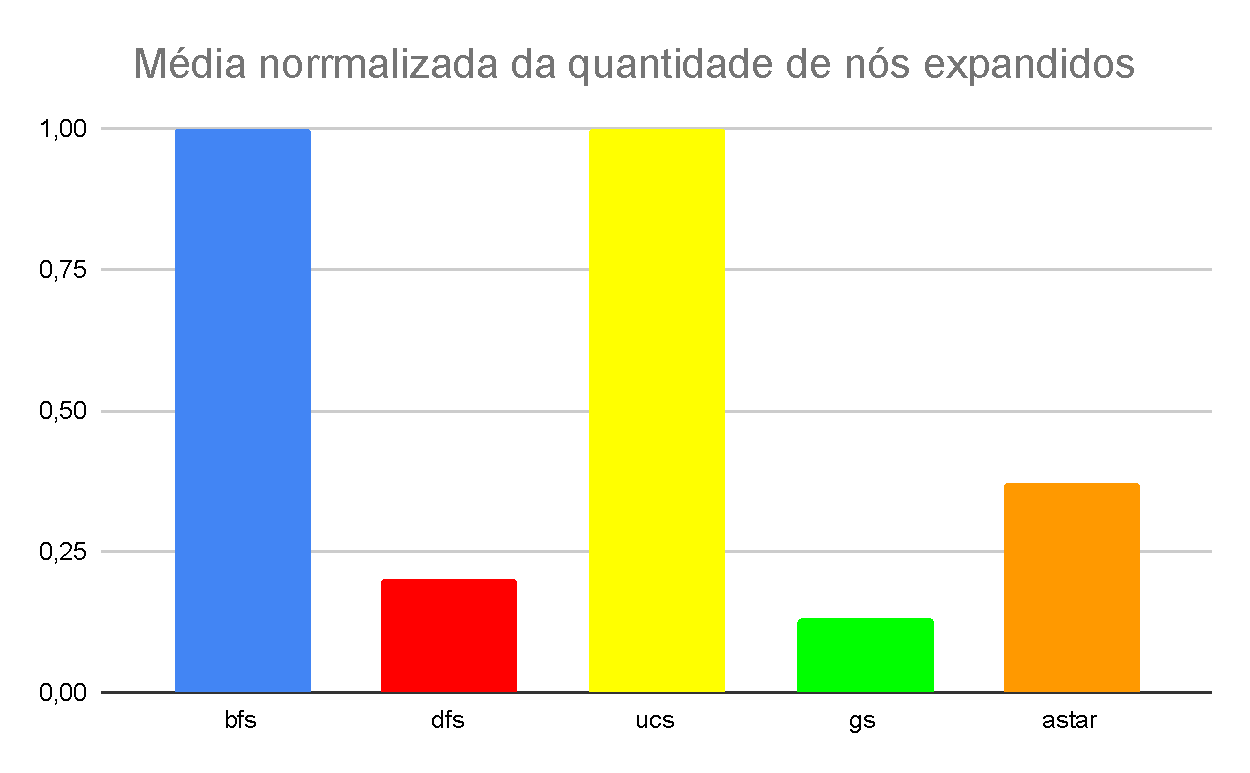
\includegraphics[width=.8\textwidth]{fig/expansao.pdf}
  \caption{Média da quantidade de nós expandidos em todos os possíveis \textit{\$scenarios} para cada \textit{\$alg}.}
  \label{fig:expansao}
\end{figure}

Uma ultima observação sobre tais resultados é de que os algoritmos \textit{ucs}
e \textit{bfs} obtiveram ótimos custo, porém há uma alta taxa de nós expandidos
e também um alto tempo de execução, vide Figuras~\ref{fig:tempo} e
\ref{fig:expansao}.
Provavelmente, se os recursos computacionais não forem uma barreira, estas
duas soluções poderiam ser utilizadas a fim de minimiza o custo, assim
como mostra a Figura~\ref{fig:custo}.
Por fim, é importante destacar os recursos do sistema responsável
pela execução dos testes.
Tratas-se de uma máquina com CPU Intel core i5, 8GB RAM, sistema operacional
Ubuntu 18.04.

\subsection{Comparação multi fatores}

Os gráficos contidos nas Figuras~\ref{fig:tempo-custo},
\ref{fig:expansao-custo} e \ref{fig:tempo-expansao} foram obtidos a partir
do cruzamento das médias que denotam as Figuras~\ref{fig:custo},
\ref{fig:tempo} e \ref{fig:expansao}.
A partir desta exibição pode-se classificar os prós e contras de cada resultado
obtido.
Mas antes da descrição da análise, por tratar-se de um gráfico de pontos
e dada a proximidade dos resultados dos algoritmos \textit{bfs} e \textit{ucs},
estes pontos se sobrepõem em todas as três figuras
\begin{figure}[hbt!]
  \centering
  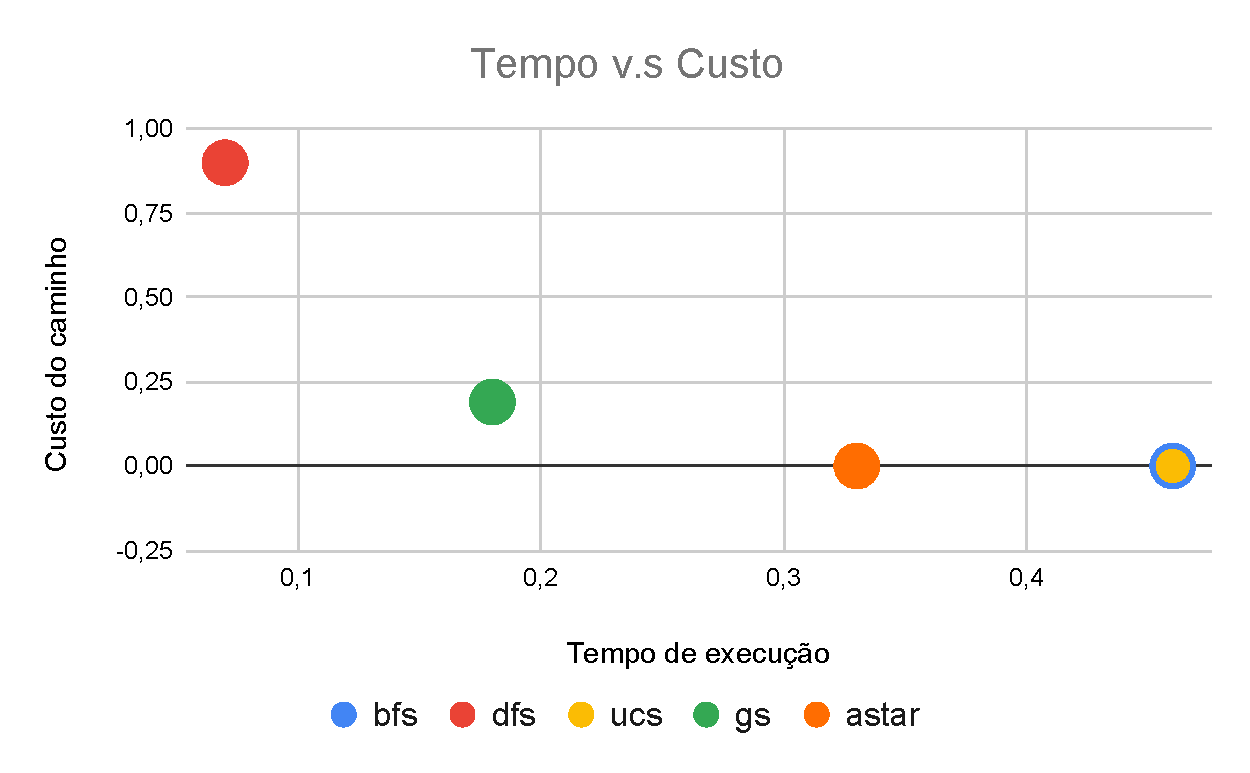
\includegraphics[width=.8\textwidth]{fig/tempo-custo.pdf}
  \caption{Comparação tempo e custo de execução}
  \label{fig:tempo-custo}
\end{figure}

\begin{figure}[hbt!]
  \centering
  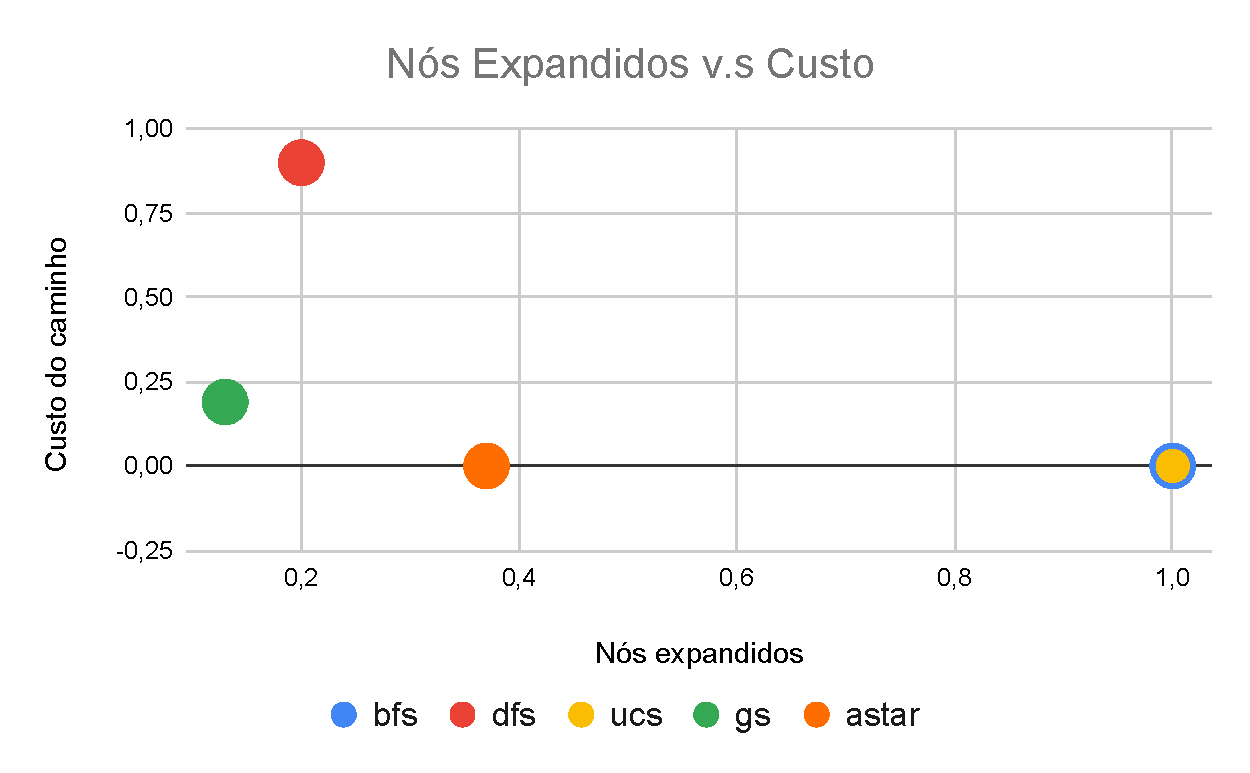
\includegraphics[width=.8\textwidth]{fig/expansao-custo.pdf}
  \caption{Comparação da quantidade de nós expandidos e o custo}
  \label{fig:expansao-custo}
\end{figure}

\begin{figure}[hbt!]
  \centering
  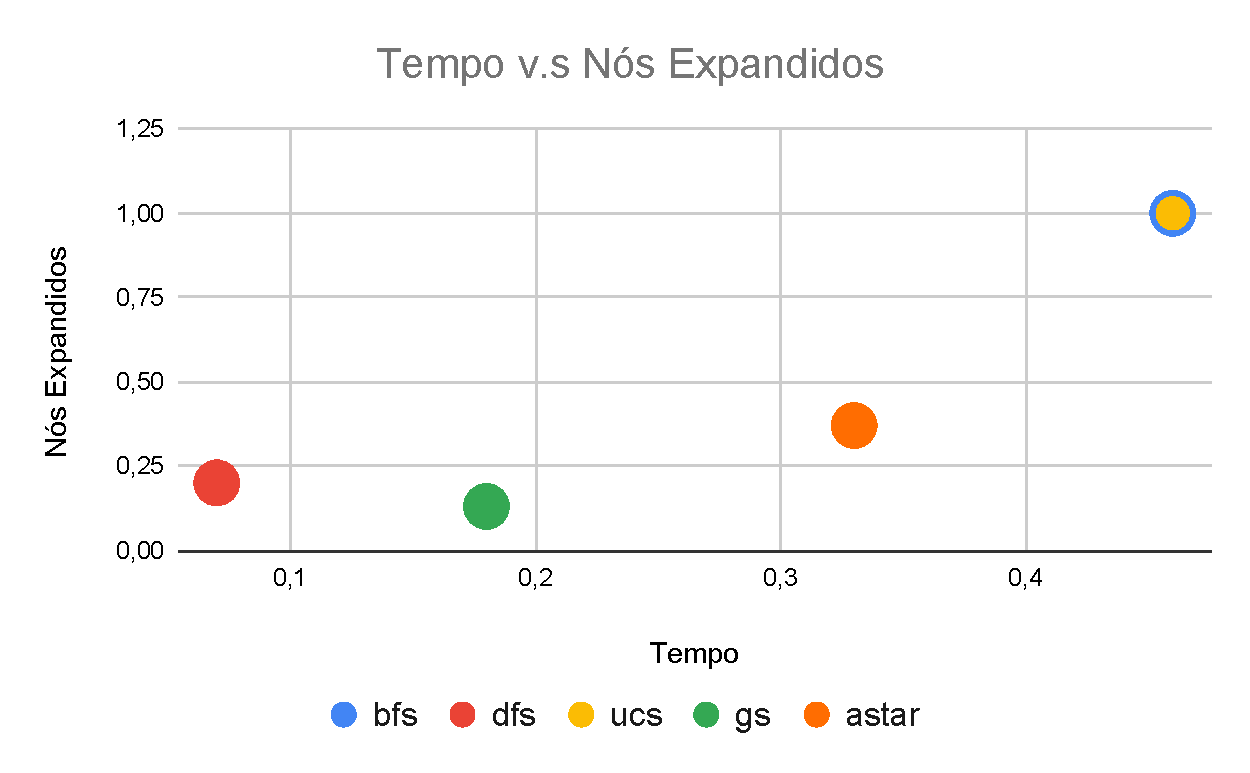
\includegraphics[width=.8\textwidth]{fig/tempo-expansao.pdf}
  \caption{Comparação tempo e quantidade de nós expandidos}
  \label{fig:tempo-expansao}
\end{figure}

Através dos gráficos de cruzamento de fatores, fica evidente que \textit{gs} é
um bom meio termo, em que pode-se combinar um bom desempenho e custos reduzidos.
Além disso, este algoritmo expande poucos nós se aproximando muito do resultado
ótimo.
Mas a observação que pode-se realizar de cada um dos gráficos de dados cruzados
é que quão mais pŕoximo do ponto $(0,0)$, melhor é o desempenho da solução.
A afirmação sobre a relação entre tempo e quantidade de nós expandidos é aferida
pela Figura~\ref{fig:tempo-expansao}, em que os pontos são dispersos de maneira
quase colinear.

\subsection{FoodHeuristic}
Uma vez que a heurística desenvolvida para o passo 7 deste trabalho deve
considerar múltiplos pontos, pensou-se em uma versão relaxada do problema
o qual apenas um ponto de comida é considerado, e desconsidera-se a existência
de obstáculos (paredes).
Ao avaliar a função heurística de determinado estado, busca-se pelo ponto de
comida mais distante, e então retorna-se a distância de manhattan entre o estado
consultado e o estado objetivo mais distante.
Esta abordagem faz com que a expansão de nós tenda a uma região do mapa, e após
consumir todos os estados objetivos daquela região, outra região será apontada
como tendência.
Tal viés é o responsável por reduzir a quantidade de nós expandidos.

\begin{figure}[hbt!]
  \centering
  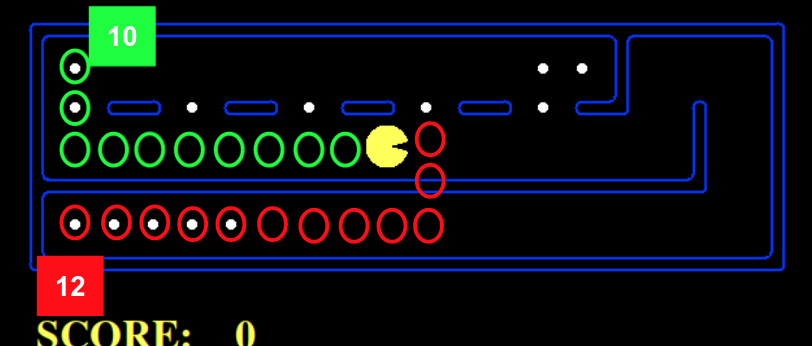
\includegraphics[width=.8\textwidth]{fig/manhattan.png}
  \caption{Distância de manhattan nas duas primeiras consultas em \textit{trickySearch}}
  \label{fig:manhattan}
\end{figure}

Figura~\ref{fig:manhattan} demonstra a consulta à função heurística no estado
inicial da fase \textit{trickySearch}.
Nela é possível observar que só há dois possíveis estados para expandir:
Aquele que aponta para a \textbf{direita} está a 12 pontos (segundo a
distância de manhattan) do nó objetivo mais longe.
Já as posição que está à esquerda do estado inicial, está à 10 pontos de
distância do estado objetivo mais distante.
Logo o estado escolhido será aquele que aponta para a esquerda.

Esta heurística é consistente e admissível, uma vez que passa pelo teste
de admissibilidade do passo 7 e também por sempre caminhar para em direção
daquele estado que optimiza o caminho sem superestimar a solução do problema
original.
A consistência é justificada pela construção do caminho, que prioriza uma direção
para que o Pac-Man caminhe.
Dessa forma, o caminhamento está na direção da optimalidade, uma vez que a
heurística implementa uma tendência de movimento para um nó objetivo.

Por fim, o resultado da execução de \textit{trickySearch} através de
\textit{foodHeuristics} expande 9551 estados.
Tal execução é dada pelo comando:
\begin{center}
  \textit{python3 pacman.py --layout trickySearch --pacman AStarFoodSearchAgent}
\end{center}

\section{Conclusão}
Em resumo, a implementação do trabalho foi muito interessante, uma vez que
conceitos já lecionados em teoria foram aplicados na prática.
Isso foi importante para dar a percepção de quão trabalhoso é o processo da
construção de soluções consistentes para sistemas de inteligência artificial,
uma vez que é necessário avaliar diversos casos e soluções.
Além disso, foi necessária a implementação de uma heurística, o que faz com que
a criatividade seja despertada.
Ainda é possível destacar que os resultados encontrados foram satisfatórios.

A principal dificuldade encontrada neste trabalho foi o desenvolvimento da
heurística, para que o valor estivesse abaixo de 10000.
Foi necessário testar duas abordagens antes da solução empregada:
uma delas utilizando a distância euclidiana média entre determinado estado e
todos os demais estados objetivos.
A outra, era apenas uma pequena mudança que avaliava a distância de manhattan
média entre um estado e todos os demais estados objetivos.

Acredito que nõa haja sugestões para trabalhos futuros, mas gostaria de deixar
um elogio a este trabalho.
Foi extremamente condizente com o que fora lecionado, além de possuir grau
de dificuldade que considero adequado, visto a qualidade das aulas e do
material disponibilizado.

% \section{References}

% Bibliographic references must be unambiguous and uniform.  We recommend giving
% the author names references in brackets, e.g. \cite{knuth:84},
% \cite{boulic:91}, and \cite{smith:99}.

% The references must be listed using 12 point font size, with 6 points of space
% before each reference. The first line of each reference should not be
% indented, while the subsequent should be indented by 0.5 cm.

\bibliographystyle{sbc}
\bibliography{sbc-template}

\end{document}
